\chapter{Metodología y método de trabajo}
\label{cap:MiMetodologia}


Se va a seguir una metodología de desarrollo en espiral: el Proceso Unificado de Desarrollo. Esta metodología consiste en la división del proyecto en cuatro etapas:
\begin{itemize}
    \item Inicio: para comenzar, se recogerán todos los requisitos y se estimará el alcance del proyecto.
    \item Elaboración: se harán prototipos de las interfaces, se diseñará el software mediante diagramas y se estimarán las iteraciones a seguir.
    \item Construcción: se escribirá el software según el resultado de la fase de elaboración, siguiendo las iteraciones calculadas. 
    \item Transición: para finalizar se probará el producto final y, si procede, se dará fin al desarrollo.
\end{itemize}
En toda iteración habrá una fase de pruebas para verificar que el nuevo paquete de funcionalidades se haya integrado correctamente, que ninguno de los componentes anteriores se haya visto afectado de forma negativa, y a fin de asegurar la seguridad y calidad del producto hasta esa fecha.

Para la obtención y clasificación de los requisitos, se optará por varias metodologías:
\begin{itemize}
	\item Observación activa: se estudiará el entorno de trabajo del usuario final. Para ello, se realizó una sesión en la que se monitorizó a un usuario usando una de las herramientas descritas en el capítulo Aplicaciones existentes, preguntándole sus opiniones sobre algunas de las características que estaba utilizando.
	\item Entrevistas: entrevistas con el usuario en las que irá evaluando el producto final de cada sprint y añadiendo o modificando características.
\end{itemize}

	
\section{Prototipos de interfaces}
En las figuras \ref{Fig:mockup_mainwindow}, \ref{Fig:mockup_nuevatarea} y \ref{Fig:mockup_informealumno} se muestran algunos de los prototipos que se hicieron en la fase de elaboración para las interfaces del programa.

\begin{figure}[h]
\centering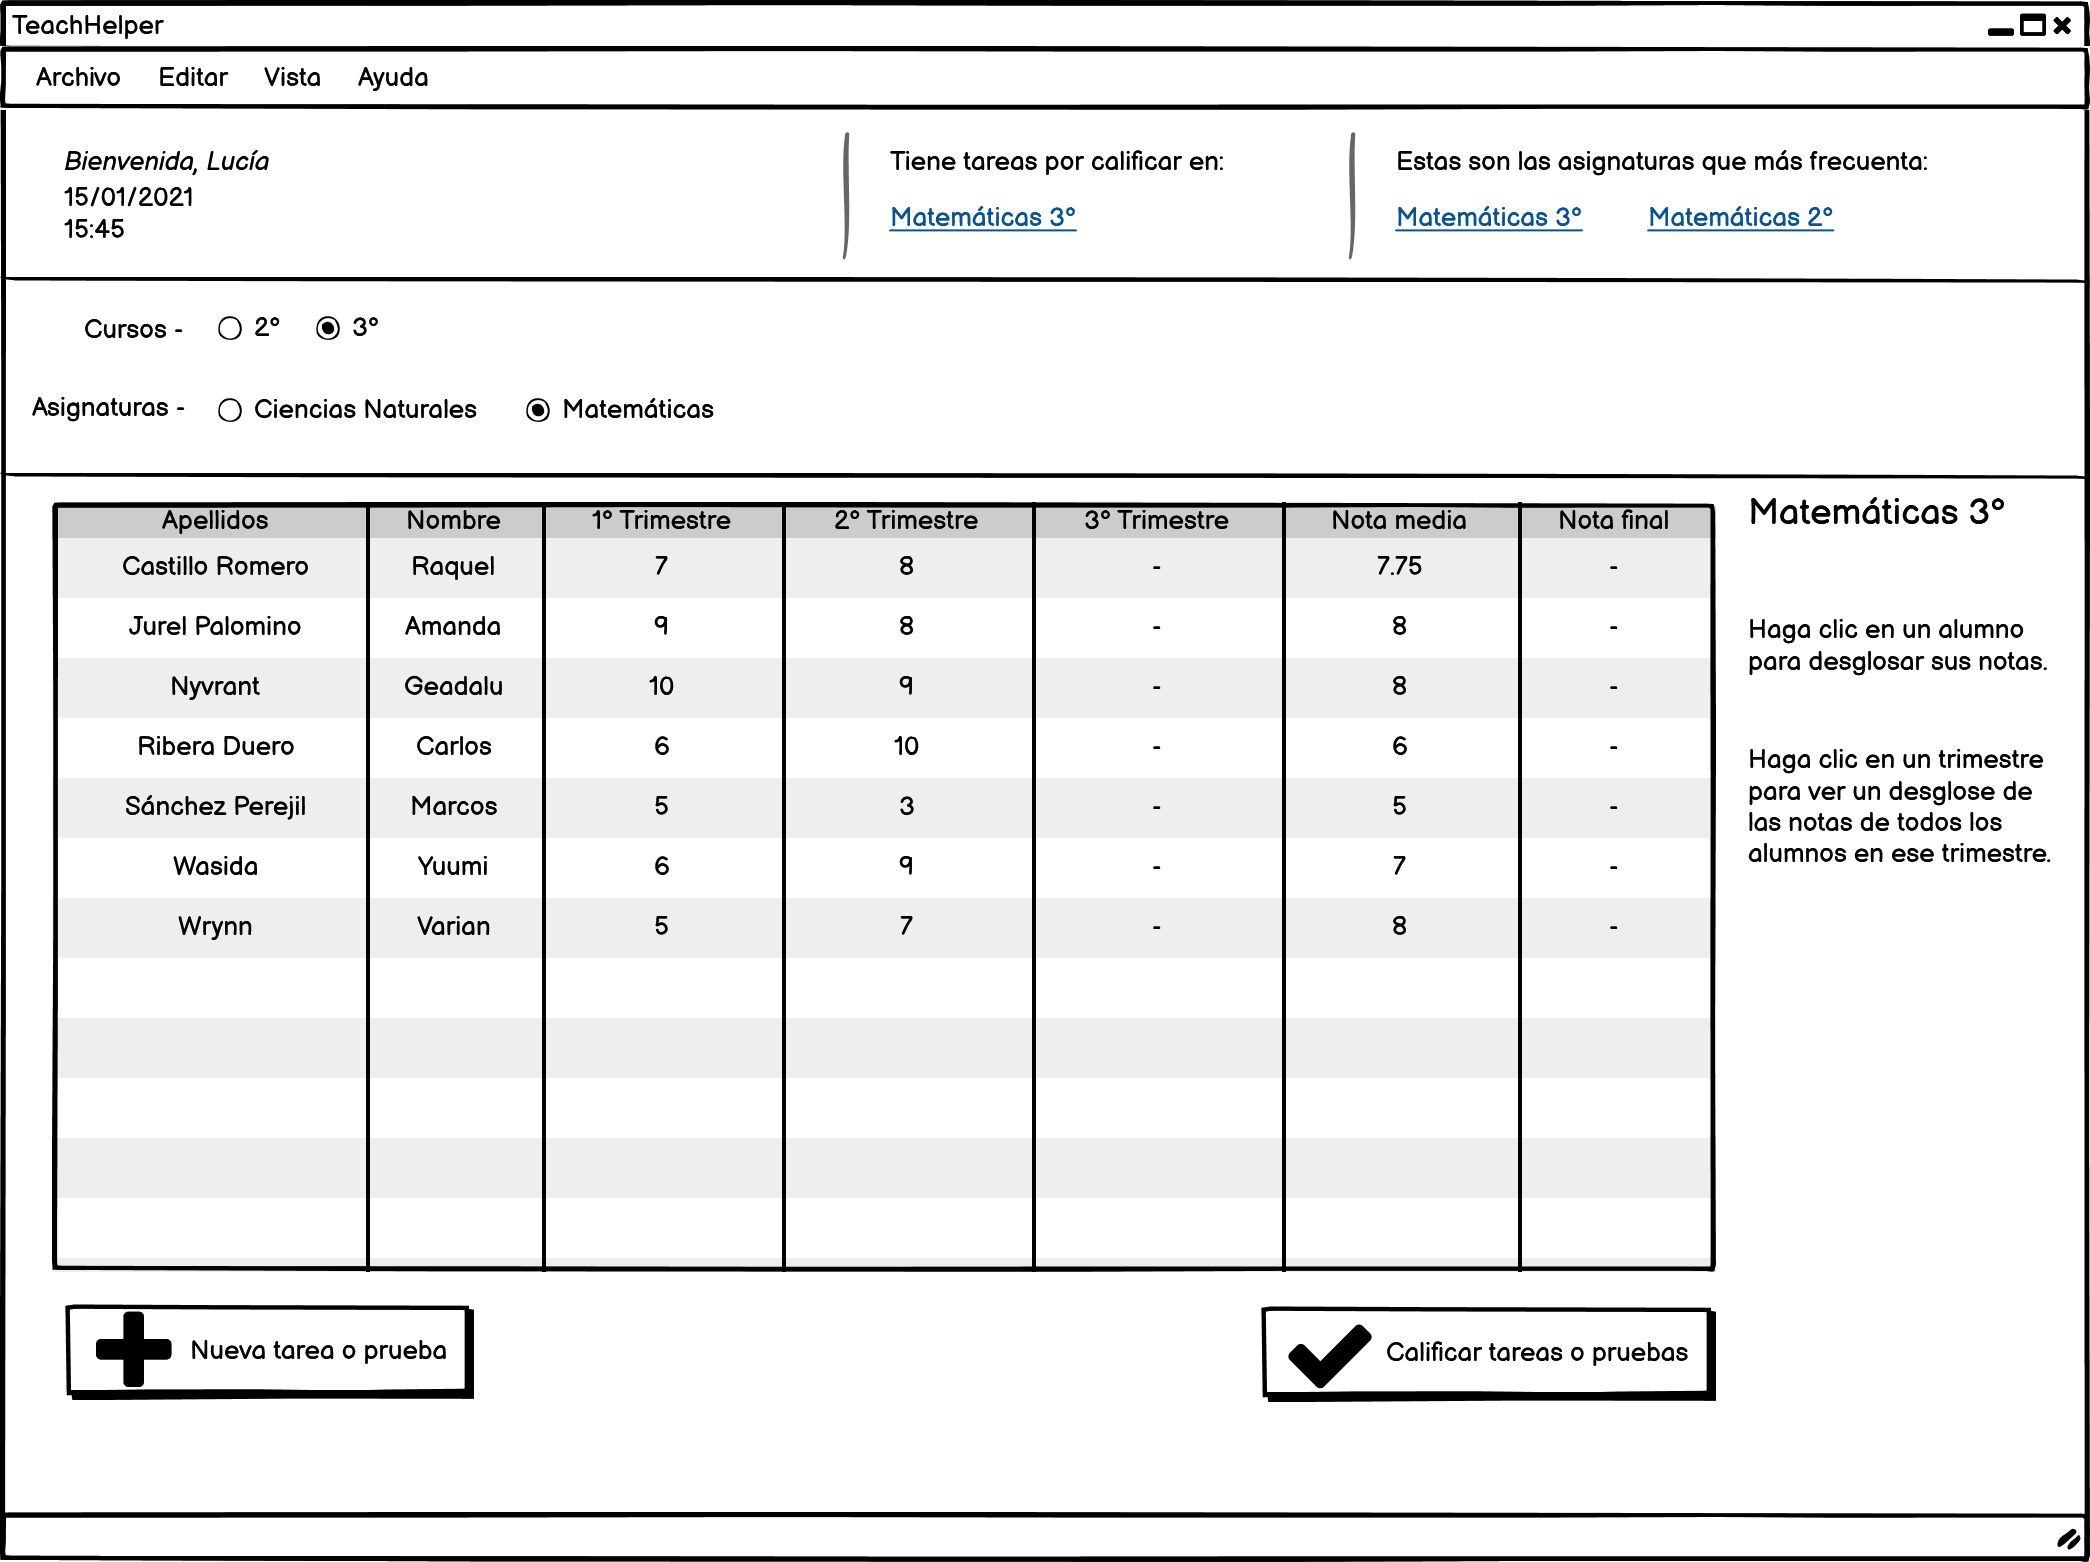
\includegraphics[width=1\linewidth]{figs/mockup_mainwindow.png}
\caption{Ventana principal.}
\label{Fig:mockup_mainwindow}
\end{figure}

\begin{figure}[h]
\centering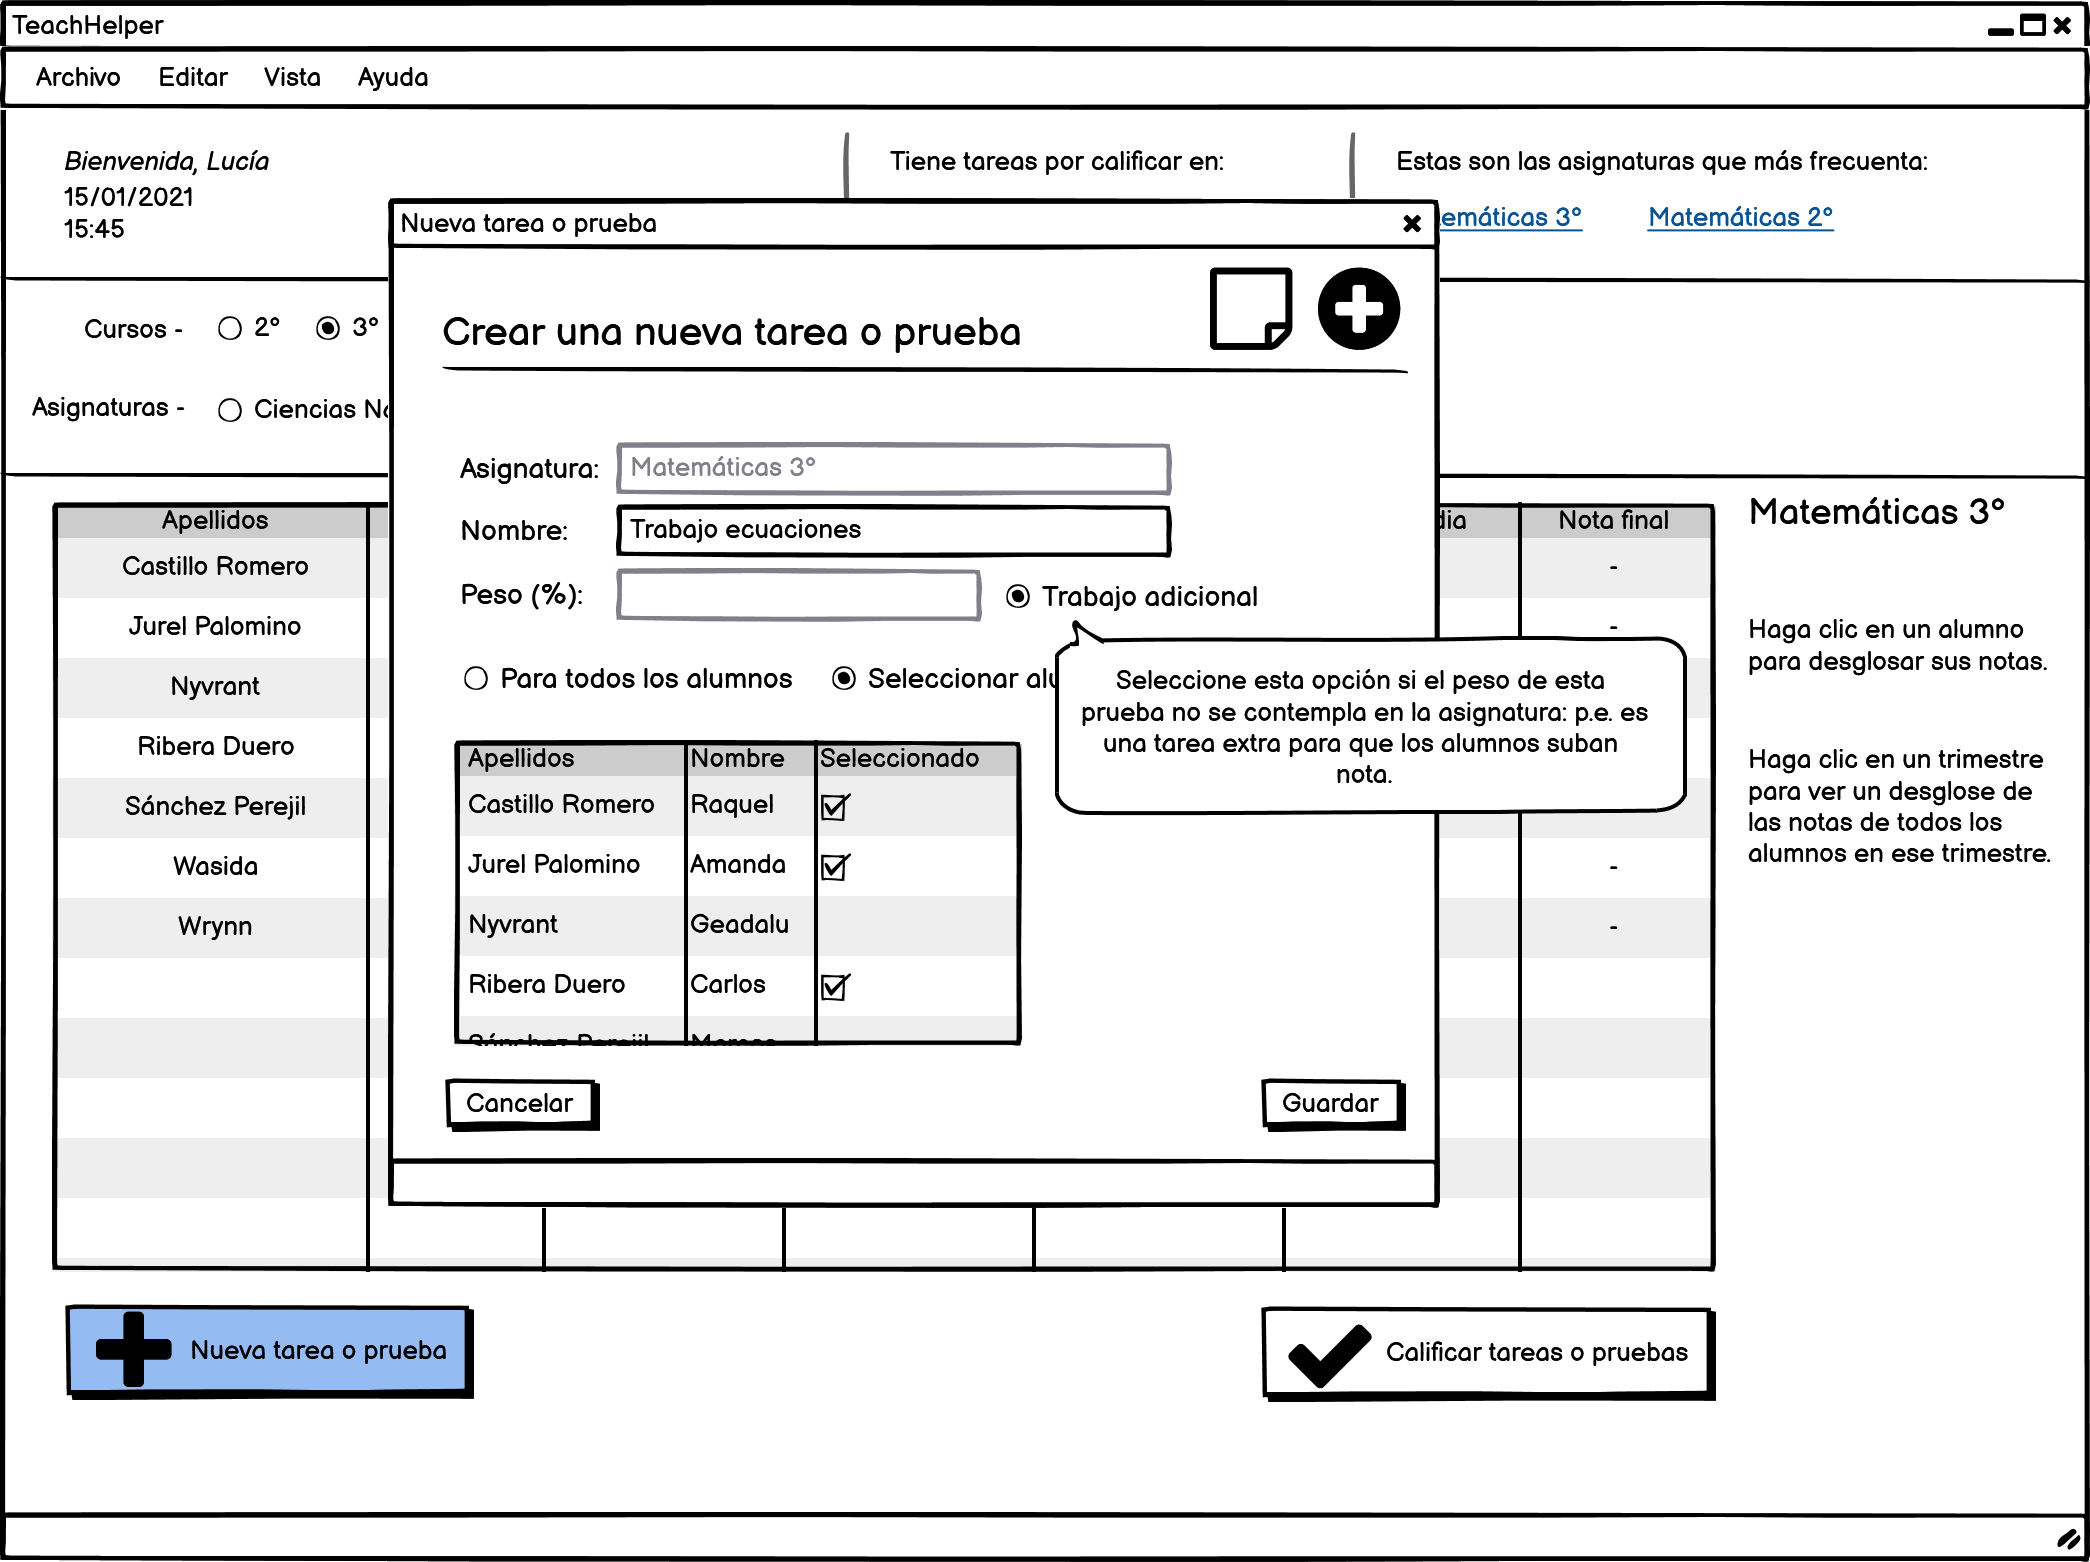
\includegraphics[width=1\linewidth]{figs/mockup_nuevatarea.png}
\caption{Crear nuevas tareas o pruebas.}
\label{Fig:mockup_nuevatarea}
\end{figure}

\begin{figure}[h]
\centering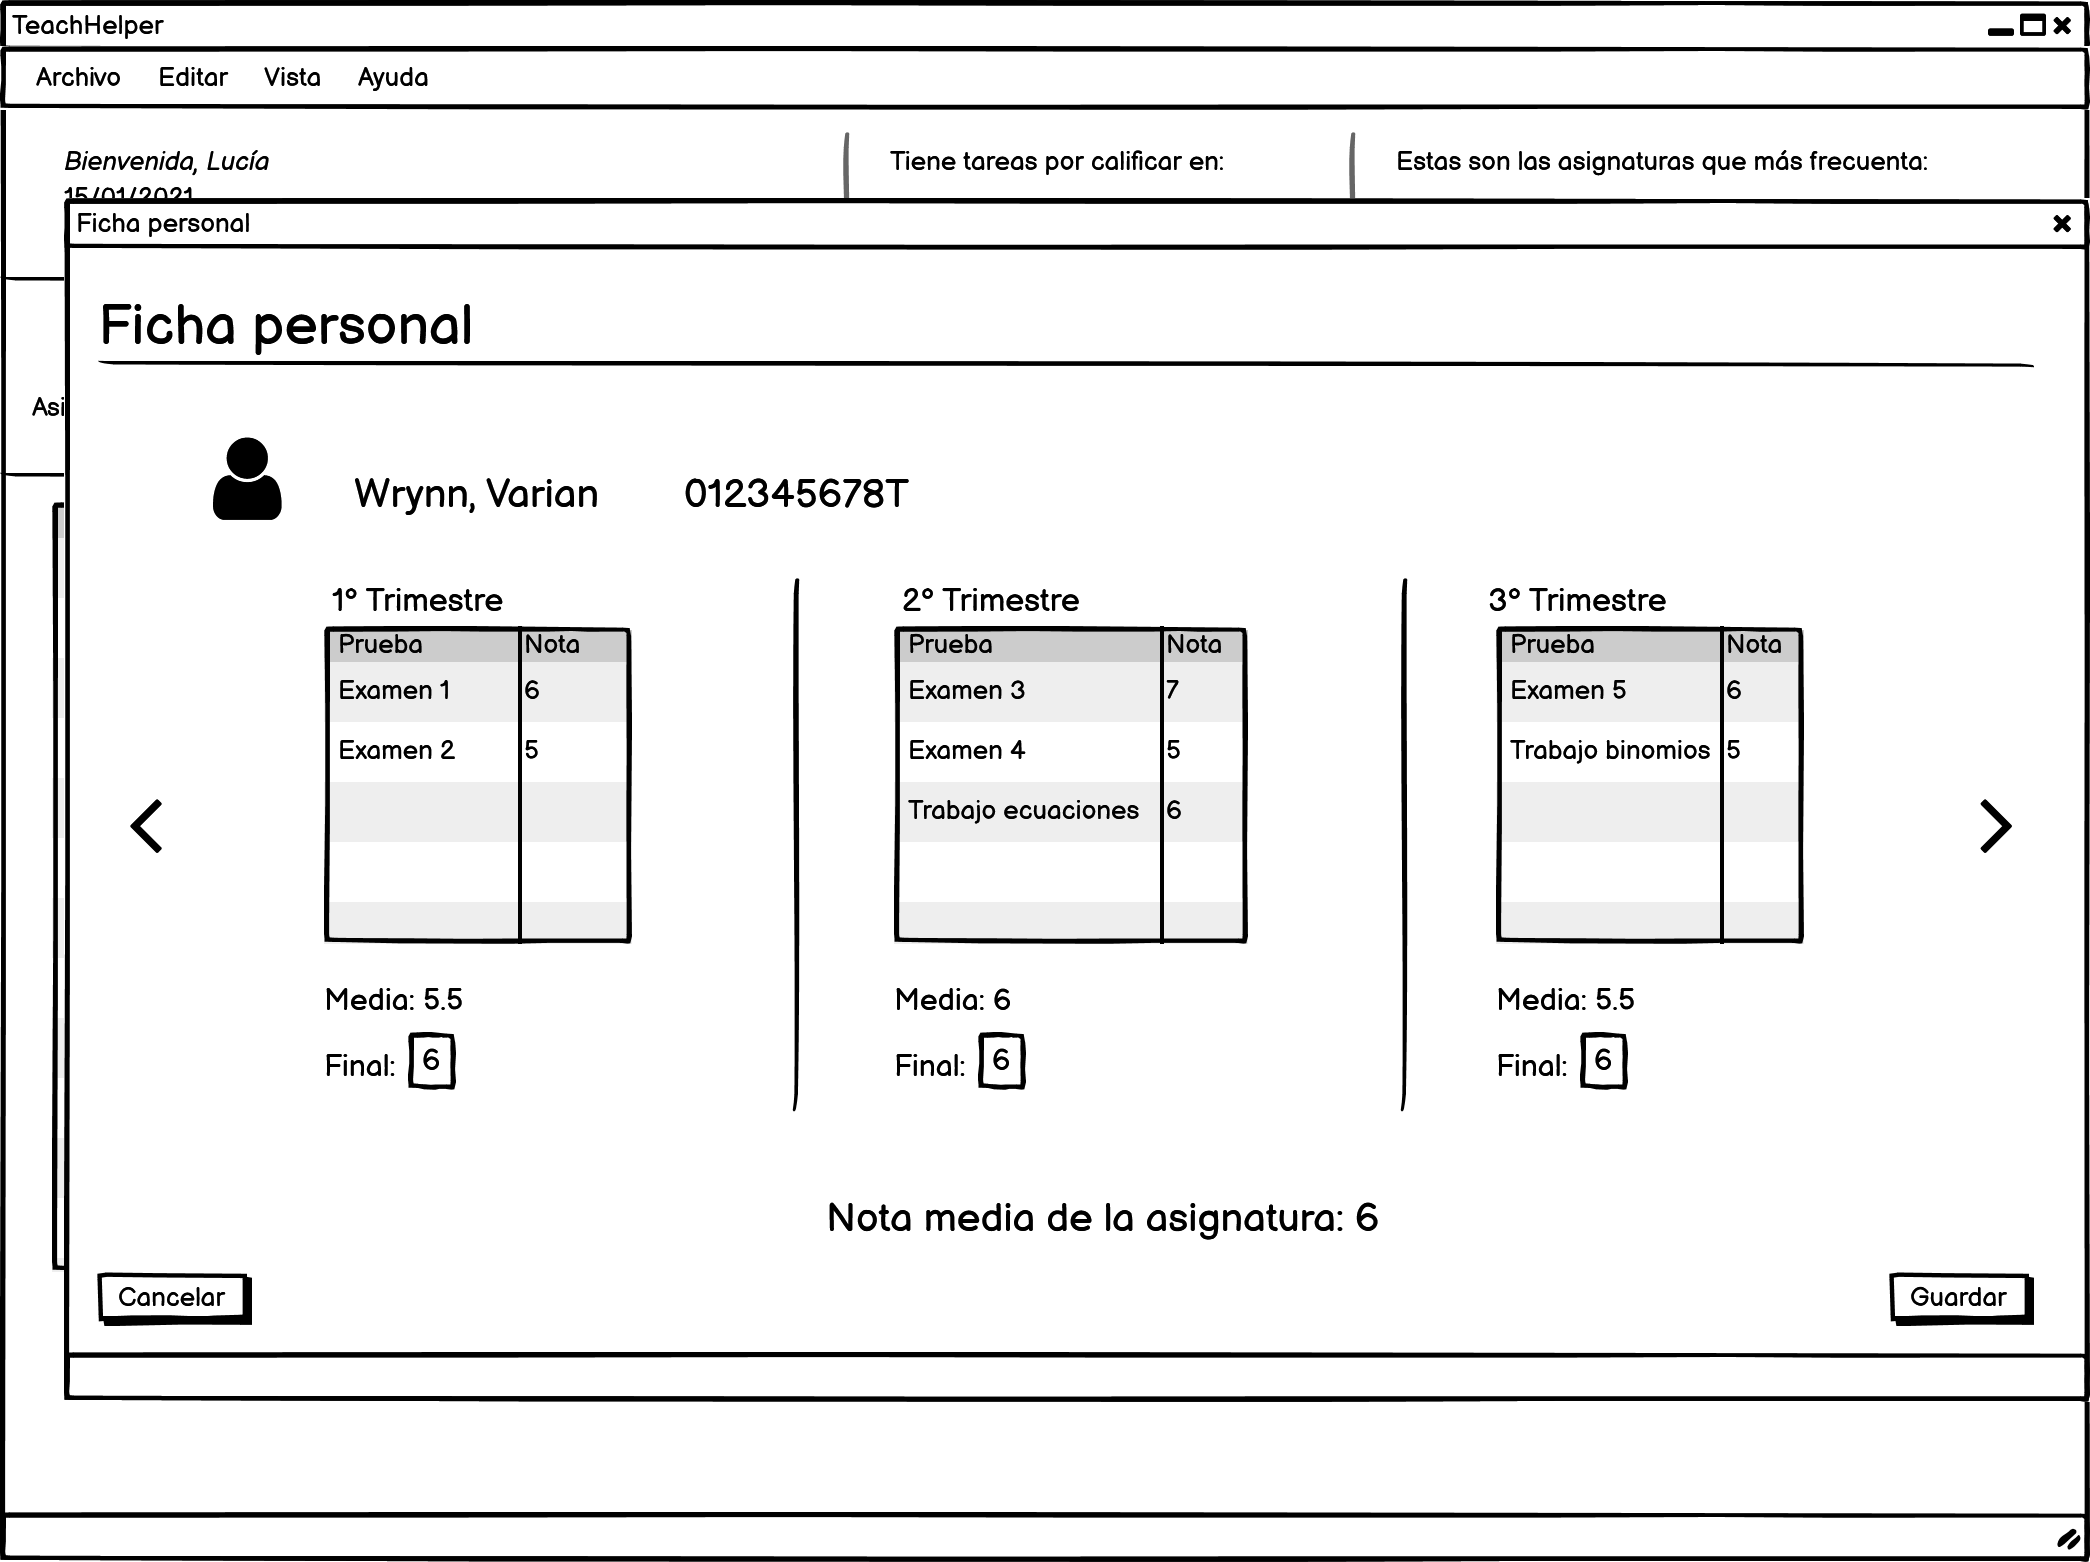
\includegraphics[width=1\linewidth]{figs/mockup_informealumno.png}
\caption{Informe del alumnado.}
\label{Fig:mockup_informealumno}
\end{figure}




\section{Sprints}


\subsection{Primer sprint - 2octub/1nov}

En el primer sprint (2 octubre 2020 - 1 noviembre 2020) se realizaron los diseños de la aplicación con la herramienta Balsamiq Wireframes. Estos diseños han ido cambiando varias veces a lo largo de este primer sprint. Además, se realizó el primer diseño de la base de datos (ver figura \ref{Fig:db_definition1}).

\begin{figure}[h]
\centering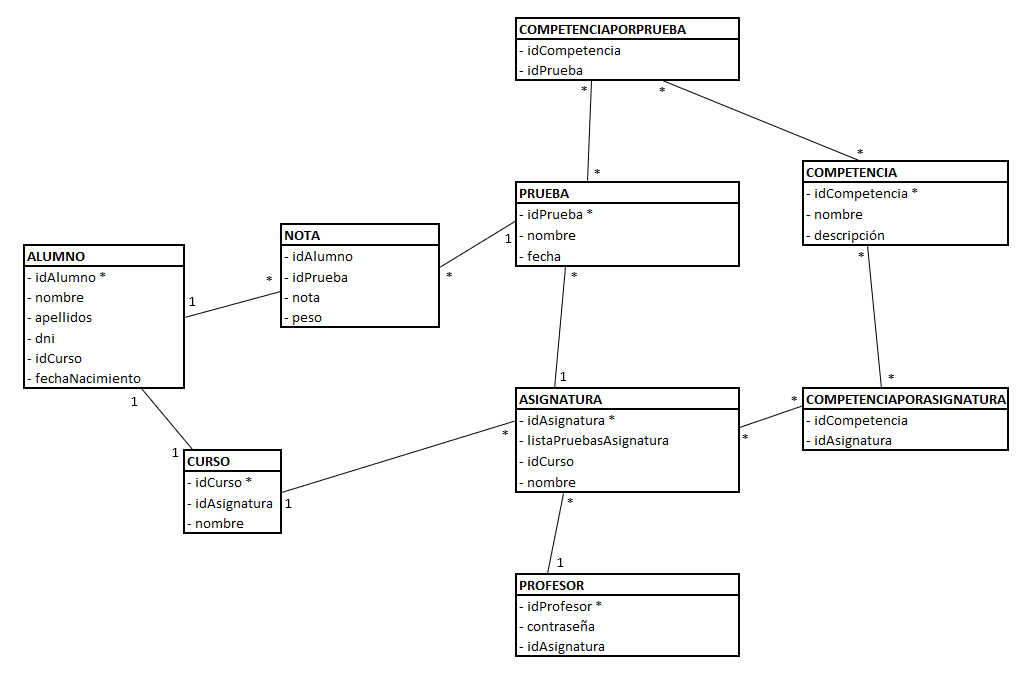
\includegraphics[width=1\linewidth]{figs/DB_Definition_1.png}
\caption{Primera definición de la base de datos.}
\label{Fig:db_definition1}
\end{figure}

\subsection{Segundo sprint - 2nov/1dic}

En el segundo sprint (2 noviembre 2020 - 1 diciembre 2020) se hicieron los siguientes cambios:
\begin{itemize}
	\item Comienzo de la escritura de la memoria del trabajo
	\item Implementación de la base de datos
\end{itemize}

\subsection{Tercer sprint - 2dic/1ene}

En el tercer sprint (2 diciembre 2020 - 1 febrero 2021) se hicieron los siguientes cambios:
\begin{itemize}
	\item Comienzo de la implementación de la aplicación: creación de la ventana principal.
	\item Se pobla inicialmente la base de datos con datos de prueba.
\end{itemize}

\subsection{Cuarto sprint - 2feb/1mar}

En el cuarto sprint (2 febrero 2021 - 1 marzo 2021) se continuó con el desarrollo de la ventana principal. Cabe notar que en este sprint se decidió dejar las mejoras del diseño de la ventana para sprints posteriores y comenzar con el desarrollo de las funcionalidades.

\subsection{Quinto sprint - 2mar/1may}

En el quinto sprint (2 marzo 2021 - 1 abril 2021) se continuó con el desarrollo general de la aplicación.

\subsection{Sexto sprint - 2may/1jul}

El sexto sprint (2 mayo 2021 - 1 julio 2021) se dedicó a corregir y realizar pequeños desarrollos en la aplicación, que si bien no añadían nuevas funcionalidades, pulían las ya existentes.

